% !engine = xelatex
% TrueType fonts (DejaVu, shipped with TeX Live and MiKTeX) through fontspec: xelatex embeds them as
% CIDFontType2 subsets, the kind of font a deck in a .ttf theme (themes/google) carries.
\documentclass[aspectratio=169]{beamer}
\usepackage{fontspec}
\setsansfont{DejaVuSans.ttf}[
  BoldFont = DejaVuSans-Bold.ttf,
  ItalicFont = DejaVuSans-Oblique.ttf,
  BoldItalicFont = DejaVuSans-BoldOblique.ttf]
\setmainfont{DejaVuSerif.ttf}[
  BoldFont = DejaVuSerif-Bold.ttf,
  ItalicFont = DejaVuSerif-Italic.ttf]
\setmonofont{DejaVuSansMono.ttf}[Scale = 0.9]
\usetheme{Madrid}
\usepackage{tikz}
\title{TrueType Fonts}
\author{Tester}
\date{}

\begin{document}

\begin{frame}
  \titlepage
\end{frame}

\begin{frame}{Styles and Unicode}
  \begin{itemize}
    \item Regular, \textbf{bold}, \textit{oblique} and \textbf{\textit{both}}
    \item Accents: Café, naïve, Straße, Łódź, Ærøskøbing, Ωμέγα, Кириллица
    \item Ligatures stay letters: office, affine, flow
    \item Arrows and symbols: → ⇒ ± × ≤ ≥ ∞ ✓ ★ ♥
      \begin{itemize}
        \item Nested item in \texttt{monospace}
        \item {\rmfamily A serif phrase}, then sans again
      \end{itemize}
  \end{itemize}
\end{frame}

\begin{frame}{A paragraph and a block}
  Lorem ipsum dolor sit amet, consectetur adipiscing elit, sed do eiusmod tempor
  incididunt ut labore et dolore magna aliqua. Ut enim ad minim veniam, quis
  nostrud exercitation ullamco laboris nisi ut aliquip ex ea commodo consequat.

  \begin{block}{Definition}
    A \emph{TrueType} font draws its glyphs with quadratic curves; inline
    math such as $x^2 + y_i = \alpha$ still uses Computer Modern.
  \end{block}
\end{frame}

\begin{frame}[fragile]{Code and a table}
\begin{verbatim}
def area(r):
    return 3.14159 * r ** 2   # πr²
\end{verbatim}
  \begin{center}
    \begin{tabular}{lrr}
      \hline
      Font & Glyphs & Size \\
      \hline
      DejaVu Sans & 6253 & 757 kB \\
      DejaVu Mono & 3381 & 340 kB \\
      \hline
    \end{tabular}
  \end{center}
\end{frame}

\begin{frame}{Turned, stroked and scaled text}
  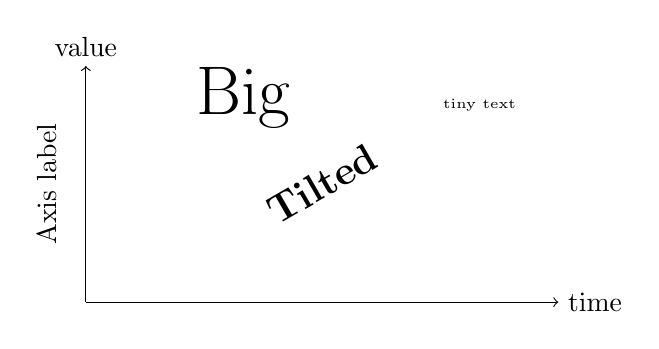
\begin{tikzpicture}
    \draw[->] (0,0) -- (6,0) node[right] {time};
    \draw[->] (0,0) -- (0,3) node[above, rotate=0] {value};
    \node[rotate=90] at (-0.5,1.5) {Axis label};
    \node[rotate=30, font=\Large\bfseries] at (3,1.5) {Tilted};
    \node[font=\tiny] at (5,2.5) {tiny text};
    \node[font=\Huge] at (2,2.6) {Big};
  \end{tikzpicture}
  \par\bigskip
  \special{pdf:literal 1 Tr 0.4 w}Outlined words\special{pdf:literal 0 Tr} and filled ones.
\end{frame}

\end{document}
